\subsection{Architecture}

Our product it made up of two parts: the control server, and the door nodes.
Our product interacts with two types of actors: Operators and Users.

The control server maintains a database of operator profiles, operator logs,
user profiles, and interaction logs.  The control server will use the operator
profiles to validate users using the operator GUI.  Every action performed in
the operator GUI will be logged in the operator logs.  Operators can create and
modify user profiles.  When a user attempts to use a door node, their identity
is checked against their user profile.  Each interaction with a door node is
recorded in a user log.

\begin{figure}[!htb]
\centering
\includegraphics[width=0.75\textwidth]{uml/architecture.png}
\caption{UML Architecture Diagram}
\label{fig:architecture-diagram}
\end{figure}

\subsection{Message Sequence Diagrams}

As seen in Figure \ref{fig:message-sequence-diagram}, all message sequences are
initiated by the Door Node sending an ACCESS\_REQUEST.  The Control Server can
reply with an ACCESS\_RESPONSE to immediately grant or deny access.  If the
Control Server doesn't have enough information to make a decision, it will send
INFORMATION\_REQUEST's until it has enough information to send an
ACCESS\_RESPONSE message.

These messages are built in a way that additional sensors could easily be added
to system.

Since there are separate Door Nodes for entrances and exits, the Control Server
can determine if a user is entering or exiting based on the Node ID.  If a Door
Node is to be used for both entering and exiting, it will be equipped with two
NFC Security Badge Readers.  The Door Node will use a separate Node ID for
interactions with each NFC Security Badge Reader.  The Control Server will view
this Door Node with two NFC Security Badge Readers as two separate Door Nodes.

When a user is entering the building, the Control Server will consult the
database to determine if the user is authorized to enter the building.  If the
the user is not authorized, the Control Server will respond with an
ACCESS\_RESPONSE message denying the user.  If the user is authorized, the
Control Server will respond with an INFORMATION\_REQUEST for the user's
temperature.  The door node will then respond with an INFORMATION\_RESPONSE
containing the user's temperature.  The Control Server will repeat the
INFORMATION\_REQUEST for temperature until a temperature not indicating a fever
is received, or the maximum number of tries is reached.  The Control Server
will then respond with an ACCESS\_RESPONSE message denying the user if it is
determined they might have a fever or granting access to the user if their
temperature is normal.  The Control server will then update the database.

When a user is exiting the building, the Control Server will immediately respond
with an ACCESS\_RESPONSE message granting access to the user.  The Control
Server will then use this information to update the database.

\begin{figure}[!htb]
\centering
\includegraphics[width=0.75\textwidth]{uml/message-sequence-diagram.png}
\caption{Message Sequence Diagram}
\label{fig:message-sequence-diagram}
\end{figure}

\subsection{Communication Protocol}
\label{subsec:communication-protocol}

Our communication protocol consists of two layers: a simple transport layer that
abstracts over ThingSpeak and an application layer that carries information
specific to our system.

\subsubsection{ThingSpeak Transport Layer}

The ThingSpeak transport layer is designed to provide an interface that
functions similarly to a TCP or UDP socket but uses ThingSpeak as a backend.

The ThingSpeak transport layer uses a single ThingSpeak channel to facilitate
communication between an arbitrary number of endpoints. Each entry posted to the
channel uses two ThingSpeak fields. The first contains a transport layer header
and the second contains the application layer data.

The ThingSpeak transport layer header is encoded as string in the first field of
a ThingSpeak channel entry. It contains three fields, which are separated by a
tab character.
\begin{itemize}
    \item Source Address: A string the uniquely identifies the device from which
          the message originates.
    \item Destination Address: A string the uniquely identifies the device for
          which the message is intended.
    \item Flags: A comma separated lists of flags.
\end{itemize}

The valid message flags are listed in table \ref{tab:ts-transport-flags}.

\begin{table*}[htb]
\centering
\begin{tabular}{ c | c | m{6.0cm} }
\toprule
Name & Encoded Value & Description\\
\midrule
Connection Request & conn\_req & Indicates that the message is a connection
request. If set, any other flags and the payload are ignored.\\
\bottomrule
\end{tabular}
\caption{Transport Layer Header Flags}
\label{tab:ts-transport-flags}
\end{table*}

In order to establish a connection, a client sends message to the server to
which it wishes to connect that has the conn\_req flag set. If the server
receives the message and wishes to accept the connection it will respond with a
messages that has the conn\_req flag set.

The second field of a ThingSpeak channel entry contains the application layer
message content encoded as a base 64 string.

\subsubsection{Application Layer}

The application layer protocol consist of five different message types, which
are listed in table \ref{tab:app-layer-messages}.

All message fields are encoded with network endianness (big endian).

\begin{table*}[htb]
\begin{tabular}{ l | l | l | p{4.5cm} }
\toprule
Sender & Receiver & Message & Data Format\\
\midrule
Door Node & Control Server & ACCESS\_REQUEST &
Transaction ID \newline Account ID\\
\hline
Control Server & Door Node & ACCESS\_RESPONSE &
Transaction ID \newline Access Request Response\\
\hline
Control Server & Door Node & INFORMATION\_REQUEST &
Transaction ID \newline Information Type\\
\hline
Door Node & Control Server & INFORMATION\_RESPONSE &
Transaction ID \newline Information Type \newline Information Value\\
\hline
Control Server & Door Node & DOOR\_STATE\_UPDATE & New Sate\\
\bottomrule
\end{tabular}
\caption{Application Layer Messages}
\label{tab:app-layer-messages}
\end{table*}

All messages start with a 32 bit integer Message Type field. The possible
message types are listed in table \ref{tab:message-types}.

\begin{table*}[htb]
\centering
\begin{tabular}{@{}ll@{}}
\toprule
Value                   &   Description \\
\midrule
0x0                     &   Reserved for future use \\
0x1                     &   Access Request \\
0x2                     &   Access Response \\
0x3                     &   Information Request \\
0x4                     &   Information Response \\
0x5                     &   Door State Update \\
0x6 through 0xFFFFFFFF  &   Reserved for future use \\
\bottomrule
\end{tabular}
\caption{Message Type Values}
\label{tab:message-types}
\end{table*}

\paragraph{ACCESS\_REQUEST}
This message is sent by a door node in order to initiate an access request. The
message contains a transaction ID to identify this access request sequence. The
transaction ID is a 32 bit integer that should be unique for the door node that
is initializing the request. The message also contains the 128 bit identifier
from the NFC security badge that prompted the access request.

The format of an ACCESS\_REQUEST message is shown in figure
\ref{fig:msg-frmt-access-req}.

\begin{figure}[h]
\centering
\begin{bytefield}[bitwidth=0.03\linewidth]{32}
    \bitheader{0-31} \\
    \wordbox{1}{Message Type} \\
    \wordbox{1}{Transaction ID} \\
    \wordbox{4}{NFC Security Badge ID} \\
\end{bytefield}
\caption{Format of Access Request Message}
\label{fig:msg-frmt-access-req}
\end{figure}

\paragraph{ACCESS\_RESPONSE}
This message is sent by the control server in response to an access request. The
message contains a 32 bit transaction ID which must correspond to the ID from an
ACCESS\_REQUEST message send by the door node and a flag which indicates whether
access should be granted. Bits 33 to 63 of this message type are unused.

The format of an ACCESS\_RESPONSE message is shown in figure
\ref{fig:msg-frmt-access-resp}.

\begin{figure}[h]
\centering
\begin{bytefield}[bitwidth=0.03\linewidth]{32}
    \bitheader{0-31} \\
    \wordbox{1}{Message Type} \\
    \wordbox{1}{Transaction ID} \\
    \bitbox{1}{\tiny{Rsp.}} &
        \bitbox{31}{\color{lightgray}\rule{\width}{\height}}
\end{bytefield}
\caption{Format of Access Response Message}
\label{fig:msg-frmt-access-resp}
\end{figure}

\paragraph{INFORMATION\_REQUEST}
This message is sent by the control server when it requires more information in
order to make an access decision. The message contains a 32 bit transaction ID
and a 32 bit information type value. The possible information types are listed
in table \ref{tab:msg-info-req-types}.

The format of an INFORMATION\_REQUEST message is shown in figure
\ref{fig:msg-frmt-info-req}.

\begin{figure}[h]
\centering
\begin{bytefield}[bitwidth=0.03\linewidth]{32}
    \bitheader{0-31} \\
    \wordbox{1}{Message Type} \\
    \wordbox{1}{Transaction ID} \\
    \wordbox{1}{Information Type} \\
\end{bytefield}
\caption{Format of Information Request Message}
\label{fig:msg-frmt-info-req}
\end{figure}

\begin{table*}[htb]
\centering
\begin{tabular}{@{}ll@{}}
\toprule
Value                   &   Description \\
\midrule
0x0                     &   Reserved for future use \\
0x1                     &   Request user temperature \\
0x2 through 0xFFFFFFFF  &   Reserved for future use \\
\bottomrule
\end{tabular}
\caption{Information Request Types}
\label{tab:msg-info-req-types}
\end{table*}

\paragraph{INFORMATION\_RESPONSE}
This message is sent by a door node in response to an INFORMATION\_REQUEST
message. The message contains a 32 bit transaction ID, the 32 bit specifier for
the type of information requested (as specified in table
\ref{tab:msg-info-req-types}) and the requested data.

The format of the data returned will depend on the information type. For user
temperature information, the information payload will be 32 bits long. The first
16 bits will be a signed integer in two's complement format indicating the
ambient temperature in units of one hundredth of a degree Celsius per least
significant bit. The second 16 bits will be a signed integer in two's complement
format indicating the temperature of the user in units of one hundredth of a
degree Celsius per least significant bit.

The format of an INFORMATION\_RESPONSE message is shown in figure
\ref{fig:msg-frmt-info-resp}.

\begin{figure}[h]
\centering
\begin{bytefield}[bitwidth=0.03\linewidth]{32}
    \bitheader{0-31} \\
    \wordbox{1}{Message Type} \\
    \wordbox{1}{Transaction ID} \\
    \wordbox{1}{Information Type} \\
    \wordbox[tlr]{1}{Information Payload} \\
    \wordbox[blr]{1}{$\cdots$} \\
\end{bytefield}
\caption{Format of Information Response Message}
\label{fig:msg-frmt-info-resp}
\end{figure}

\paragraph{DOOR\_STATE\_UPDATE}
This message can be sent by the control server to a door node to provide it with
information about the state of the system. This information can be used by the
door node to decide what information to display to users. This state value is
encoded as a 32 bit unsigned integer. The possible state values are listed in
table \ref{tab:msg-door-states}.

The format of an DOOR\_STATE\_UPADTE message is shown in figure
\ref{fig:msg-frmt-door-state}.

\begin{figure}[h]
\centering
\begin{bytefield}[bitwidth=0.03\linewidth]{32}
    \bitheader{0-31} \\
    \wordbox{1}{Message Type} \\
    \wordbox{1}{Door State} \\
\end{bytefield}
\caption{Format of Door State Update Message}
\label{fig:msg-frmt-door-state}
\end{figure}

\begin{table*}[htb]
\centering
\begin{tabular}{@{}ll@{}}
\toprule
Value                   &   Description \\
\midrule
0x0                     &   Reserved for future use \\
0x1                     &   Allowing entry \\
0x2                     &   Not allowing entry \\
0x3 through 0xFFFFFFFF  &   Reserved for future use \\
\bottomrule
\end{tabular}
\caption{Door State Values}
\label{tab:msg-door-states}
\end{table*}

\subsection{Database Schema}

The Project Database, shown in figure \ref{fig:db-schema}, consists of six main
tables. The first table encountered by the system is the nfc\_and\_employee\_id
table, this table consists of all the list of valid NFC card id’s and their
corresponding employee id associated to the id’s. The employee id field is the
primary key in this table as there is only one unique valid NFC id associated to
an employee id unique to individual employees. The employee\_info table consists
information about all the employees working for the employer, this table has all
the sensitive information regarding the employee. The primary key in this table
is the employee id as it is uniquely associated with individual employees and is
also a foreign key as it is being referred from the nfc\_and\_employee\_id
table. The nodes table is a list of all the entry and exit nodes in the system,
this table consists of a list of node id’s uniquely associated to individual
entry and exit nodes in the system and also contains information about the
location of the nodes and their type. 

The access\_entry table is a log of all the employee entry and exit activity for
at least 14 days. There are no primary keys allocated to this table as all
fields would have multiple occurrences of similar values. Although, the
access\_exit table is similar to the access\_entry table and logs all employee
exit activity for at least 14 days, it is generated and populated by the
access\_entry table and doesn’t have a unique field associated to the table.
Lastly, the admin\_log table contains data regarding any activity performed on
the GUI by employees with admin access. Similar to the other activity log tables
in the database such as the access\_entry and access\_exit tables, the
admin\_log table doesn’t have a unique field either as there are many values
duplicated in every column. 

\begin{figure}[!htb]
\centering
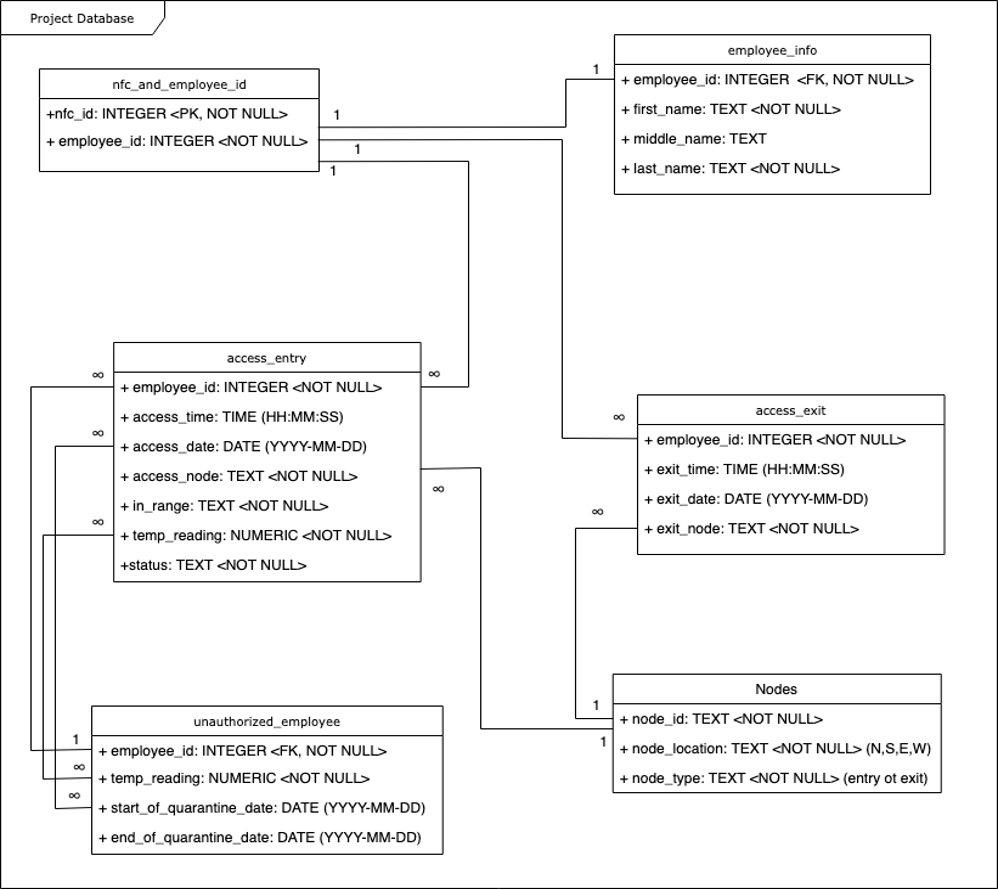
\includegraphics[width=\textwidth]{images/db-schema.png}
\caption{Database Schema}
\label{fig:db-schema}
\end{figure}

